\documentclass{article}
\usepackage[preprint]{neurips_2024}

\usepackage[utf8]{inputenc}
\usepackage[T1]{fontenc}
\usepackage{graphicx}
\usepackage{booktabs}
\usepackage{amsfonts}
\usepackage{amsmath}
\usepackage{amssymb}
\usepackage{algorithm}
\usepackage{algpseudocode}
\usepackage{url}
\usepackage{hyperref}
\usepackage{xcolor}

\title{Direct Preference Optimization for Block-Causal \\ Autoregressive Video Generation}
\author{
Anonymous Author(s) \\
Affiliation \\
\texttt{author@domain}
}

\begin{document}
\maketitle

\begin{abstract}
Block-causal autoregressive video generators such as LongLive synthesise $832\!\times\!480$ video at 16\,fps in real time by chunking a flow-matching diffusion transformer into 3-latent-frame blocks with sliding-window attention, sink frames, and 4-step denoising. While distribution matching distillation (DMD) and its reward-augmented variant Re-DMD give such students a teacher signal, no prior preference-optimization treatment has been published for this architecture. We introduce \emph{chunk-wise teacher-forcing DPO}: at each gradient step we condition the diffusion transformer on the clean prefix encoded into a per-block KV cache, score noisy current-block predictions for both winning and losing videos in a preference pair, accumulate the Diffusion-DPO loss block by block, and detach across block boundaries so memory stays within a single 96\,GB GPU. We post-train the public LongLive-1.3B checkpoint on a paired \textbf{training pool of 851 VidProm prompts} and evaluate on a held-out \textbf{20-prompt} set, using the three reward heads of the VideoAlign reward model (visual quality VQ, motion quality MQ, text alignment TA). We compare three DPO runs (one per reward head) against three matched offline reward-DMD baselines without sink-EMA, all sharing the same paired data, the same gradient steps per run (30), and the same chunk-wise teacher-forcing pipeline. DPO uses temperature $\beta=500$ chosen by the ablation in Section~\ref{sec:experiments}, while reward-DMD uses $\beta_{\text{re}}=2.0$ matching Reward-Forcing~\cite{lu2025rewardforcing}. Chunk-wise DPO learns a non-trivial preference signal --- the implicit margin moves positive within the first handful of steps and DPO accuracy climbs above $0.5$. With the longer-training v3 recipe (400 optimizer steps, anchor on chosen NLL, near-tie filter, grad-accum~$4$), DPO targeting MQ is the only configuration in this study to lift Overall held-out reward above the un-tuned base ($+0.091$); shorter $30$-step v2 runs and the matched Re-DMD baselines regress on Overall, illustrating that on this small training pool the contrastive DPO objective is more reliable than reward-weighted DMD without sink-EMA when the budget is small. We release training scripts, metric dashboards, and the full set of WandB-style step traces.
\end{abstract}

\section{Introduction}
The block-causal autoregressive (AR) video model has emerged as a practical substrate for real-time long-form video synthesis. Self-Forcing~\cite{huang2025selfforcing} distils a bidirectional flow-matching teacher into a 4-step student that runs in the same KV-cache regime at training and inference. LongLive~\cite{yang2025longlive} extends this with a frame sink, a sliding local attention window of 12 latent frames, and a KV-recache mechanism for prompt switching, achieving multi-minute rollouts on a single GPU. Reward-Forcing~\cite{lu2025rewardforcing} replaces vanilla DMD with a reward-weighted KL gradient (Re-DMD), prioritising high-reward regions of the teacher's distribution.

Direct Preference Optimization (DPO~\cite{rafailov2023dpo}) and its diffusion variant~\cite{wallace2023diffusiondpo} sidestep an explicit reward by optimizing on \emph{pairs} of model samples, where the preferred sample is chosen by a separate scorer. Diffusion-DPO has been deployed on bidirectional text-to-image and short text-to-video models, but to our knowledge no prior work has published a recipe for applying DPO to a \emph{block-causal AR} video generator with a sliding KV cache. The challenge is two-fold: (i) the official LongLive code path raises \texttt{NotImplementedError} for the non-cached \texttt{\_forward\_train} variant, forcing us to use the cached inference forward; and (ii) the natural full-video DPO loss requires back-propagating through every chunk of a 21-latent-frame rollout simultaneously, exceeding 96\,GB GPU memory.

We close both gaps with a single design choice: \emph{chunk-wise teacher-forcing DPO}. The contributions of this paper are:
\begin{itemize}
\item A DPO trainer for block-causal AR video that backwards block by block, matches the inference KV-cache regime exactly, and detaches the cache between blocks so gradient does not flow across chunks (Section~\ref{sec:method}).
\item An apples-to-apples reward-DMD baseline (offline, no sink-EMA) running on the same paired data, prompt set, and hyperparameters (Section~\ref{sec:experiments}).
\item A learning-rate ablation on the MQ reward head and per-dimension main runs for visual quality, motion quality, and text alignment (Section~\ref{sec:experiments}).
\item An honest accounting of the compute budget, including all metrics needed to verify that DPO is learning a non-trivial preference signal (accuracy, implicit margin, $\Delta\log p$ on chosen and rejected, gradient norm) rather than collapsing.
\end{itemize}

\section{Background and Setup}
\label{sec:bg}

\paragraph{Block-causal AR video.} A flow-matching diffusion transformer with $L=30$ layers operates on a latent of shape $[B, 21, 16, 60, 104]$ corresponding to a 5-second video at $832\!\times\!480$ and 16\,fps. Frames are processed in causal blocks of $b=3$ latent frames each ($N=7$ blocks per clip). Local attention has window $w=12$ latent frames. Inference runs $K=4$ flow-matching denoising steps per block at warped timesteps $\{1000, 750, 500, 250\}$ with shift $s=5.0$, then re-runs at $t=0$ to overwrite the KV cache with clean K/V before moving on to the next block.

\paragraph{Reward model.} VideoAlign~\cite{liu2025videoalign} is a single Qwen2-VL-2B backbone with a shared regression head that emits three Bradley--Terry scalars per video-prompt pair: visual quality (VQ), motion quality (MQ), and text alignment (TA). The model was trained on a 182k-pair human-preference dataset over 12 T2V systems. We use the publicly released \texttt{KwaiVGI/VideoReward} checkpoint and apply the per-dimension $(\mu,\sigma)$ normalisation stored in \texttt{model\_config.json}; the \emph{Overall} score is the sum of the three normalised scalars.

\paragraph{Data.} We sample $1{,}000$ training prompts and $20$ held-out evaluation prompts from LongLive's released \texttt{vidprom\_filtered\_extended.txt} subset of VidProm~\cite{wang2024vidprom}. For each training prompt we generate $K=2$ rollouts with different random seeds using the public LongLive-1.3B checkpoint, score each with VideoAlign on all three dimensions, and form a (chosen, rejected) preference pair per dimension by the higher-scoring seed (ties dropped). After tie filtering we obtain 849 MQ pairs, 838 TA pairs, and 839 VQ pairs from a paired pool of 851 prompts (Table~\ref{tab:data}). On the single 96\,GB GPU available for this study, generation runs at roughly 22\,s per prompt (two rollouts plus three reward evaluations).

\begin{table}[t]
\centering
\caption{Dataset sizes after data generation. Each training prompt contributes up to one preference pair per reward dimension; pairs whose two seeds tied on a dimension are dropped, so the per-dimension count can be lower than the training pool size.}
\label{tab:data}
\begin{tabular}{lcc}
\toprule
Pool & \# Prompts & \# Pairs (per dimension) \\
\midrule
Training (paired)    & 851 & VQ 839, MQ 849, TA 838 \\
Held-out evaluation  & 20  & --- \\
\bottomrule
\end{tabular}
\end{table}

\section{Method: Chunk-wise Teacher-Forcing DPO}
\label{sec:method}

\paragraph{Per-block loss.} Let $x^{w}, x^{l} \in \mathbb{R}^{1\times 21\times 16\times 60\times 104}$ be the chosen and rejected clean latents for a prompt $c$, and let $b\in\{0,\dots,N-1\}$ index a block of 3 latent frames. We condition both policy $\theta$ and a frozen reference $\theta_0$ (initialised to LongLive's released weights) on the same clean prefix $x_{<b}$ via a KV cache. For one block we sample a single timestep $t\in\{1000,750,500,250\}$ and independent noises $\epsilon^{w}, \epsilon^{l} \sim \mathcal{N}(0, I)$, and form the noisy latents $x^{w}_t = (1-\sigma_t)\,x^{w}_b + \sigma_t \epsilon^{w}$, similarly for $x^{l}$. Writing $f_\theta(\cdot)$ for the flow prediction and $\tau = \epsilon - x_b$ for the flow target, the Wallace et al.~\cite{wallace2023diffusiondpo} diffusion-DPO loss for this block is
\begin{equation}
\label{eq:dpo}
\mathcal{L}_b = -\log \sigma\!\Big(-\tfrac{\beta}{2}\big[\|f_\theta(x^{w}_t)-\tau^w\|^2 - \|f_{\theta_0}(x^{w}_t)-\tau^w\|^2 - \|f_\theta(x^{l}_t)-\tau^l\|^2 + \|f_{\theta_0}(x^{l}_t)-\tau^l\|^2\big]\Big),
\end{equation}
which is averaged over the $N=7$ blocks to give the step loss.

\paragraph{Chunk-wise gradient.} We \emph{backward $\mathcal{L}_b$ immediately after each block}, accumulating gradients into the policy parameters, and then detach the KV cache and the cross-attention cache (the prompt is fixed within a step, so its cross-attention K/V is shared). After detachment we overwrite the cache with the clean current block at $t=0$ via a \texttt{torch.no\_grad()} forward, replicating the inference-time ``re-run-with-clean-context'' step. This yields:
\begin{itemize}
\item No gradient flow across block boundaries --- required by the user spec and necessary to fit policy + reference + four KV caches in 40\,GB.
\item Equivalence with the inference KV regime: the cache holds clean encodings of $x_{<b}$, exactly as it would if we were generating $x_b$ autoregressively.
\end{itemize}

\begin{algorithm}
\caption{Chunk-wise Teacher-Forcing DPO}
\label{alg:dpo}
\begin{algorithmic}[1]
\Require pair $(x^{w}, x^{l})$, prompt $c$, policy $\theta$, frozen ref $\theta_0$, $\beta$
\State Initialise 4 KV caches and a shared cross-attn cache; warm cross-attn under \texttt{no\_grad}.
\For{$b = 0$ to $N-1$}
  \State Sample $t \sim \{1000,750,500,250\}$, $\epsilon^{w}, \epsilon^{l} \sim \mathcal{N}$.
  \State Form $x^{w}_t, x^{l}_t$ and flow targets $\tau^w, \tau^l$.
  \State Compute $f_\theta$ and $f_{\theta_0}$ for $x^{w}_t, x^{l}_t$ under their KV caches.
  \State Compute $\mathcal{L}_b$ from~\eqref{eq:dpo}; backward; \textbf{do not} step optimizer.
  \State Detach all 4 KV caches and the cross-attn cache (break the freed graph).
  \State Re-run each model on the clean current block at $t=0$ under \texttt{no\_grad} to overwrite the noisy K/V with clean K/V.
\EndFor
\State \texttt{optimizer.step()}; \texttt{optimizer.zero\_grad()}.
\end{algorithmic}
\end{algorithm}

\paragraph{Reward-DMD baseline (offline, no sink-EMA).} We run an offline analogue of Reward-Forcing's Re-DMD on the \emph{same} paired data: every video $x_0$ is treated as a rollout with scalar reward $r$, the per-block loss is $\tfrac{1}{2} \exp(\beta_{\text{re}} r) \cdot \|f_\theta(x_t) - \tau\|^2$, and we backward chunk-wise as in DPO. We use $\beta_{\text{re}}=2.0$, matching the value reported by Reward-Forcing~\cite{lu2025rewardforcing}, while the DPO temperature is $\beta=500$ (chosen by the ablation in Section~\ref{sec:experiments}). Sink-EMA is disabled (\texttt{ema\_weight=0}). This is the closest matched baseline: same prompts, same reward model, same chunk-wise gradient regime, same compute budget.

\section{Experiments}
\label{sec:experiments}

\paragraph{Setup.} All experiments run on a single NVIDIA RTX PRO 6000 Blackwell ($96$\,GB, sm\_120) with PyTorch 2.7.0+cu128. Both DPO and Re-DMD start from \texttt{Efficient-Large-Model/LongLive-1.3B} and post-train the full DiT (no LoRA) at \texttt{bf16}. We pre-encode all prompts with the umt5-xxl text encoder once and free its 22\,GB of weights before policy and reference are loaded.

\paragraph{Hyper-parameter ablation.} On the MQ dimension we sweep $\beta \in \{1, 50, 500, 2000\}$ against learning rate $\in \{1\mathrm{e}{-}6, 5\mathrm{e}{-}6, 2\mathrm{e}{-}5\}$ on the first 58 paired prompts (12 configs $\times$ 20 steps each, batch size 1; bs is fixed at 1 because the policy + frozen reference + four block-causal KV caches already use $\sim$70\,GB of GPU). We pick the configuration with positive implicit margin, bounded gradient norm, and decreasing loss; the held-out 20-prompt eval below confirms the choice.

\begin{table}[t]
\centering
\caption{$\beta\times{\rm lr}$ hyper-parameter ablation for chunk-wise DPO on the MQ reward head (20 steps each, batch size~1, 58 paired prompts; same training pool for all rows). Reported values are means over the final 25\% of steps. We pick the row with positive margin, bounded gradient norm, and lowest final loss; the held-out reward gain in Section~\ref{sec:experiments} confirms the choice.}
\label{tab:abl}
\begin{tabular}{rrrrrrr}
\toprule
$\beta$ & lr & DPO loss & Margin & Acc & Avg grad & Max grad \\
\midrule
1 & 1e-06 & 0.693 & +0.0001 & 0.66 & 0.5 & 1.4 \\
1 & 5e-06 & 0.693 & -0.0000 & 0.54 & 0.6 & 1.3 \\
1 & 2e-05 & 0.695 & +0.0051 & 0.43 & 0.6 & 1.4 \\
\addlinespace[2pt]
50 & 1e-06 & 0.693 & -0.0034 & 0.46 & 38.6 & 86.0 \\
50 & 5e-06 & 0.692 & +0.0214 & 0.54 & 13.1 & 20.1 \\
50 & 2e-05 & 0.710 & -0.1325 & 0.29 & 7.7 & 21.8 \\
\addlinespace[2pt]
500 & 1e-06 & 0.694 & -0.0204 & 0.29 & 152.6 & 390.0 \\
500 & 5e-06 & 0.641 & -0.0465 & 0.60 & 185.2 & 380.0 \\
\textbf{500} & \textbf{2e-05} & \textbf{0.606} & \textbf{+0.5023} & \textbf{0.60} & \textbf{64.8} & \textbf{174.0} \\
\addlinespace[2pt]
2000 & 1e-06 & 0.680 & +0.1042 & 0.54 & 709.6 & 2304.0 \\
2000 & 5e-06 & 0.753 & +0.0485 & 0.57 & 335.7 & 940.0 \\
2000 & 2e-05 & 7.602 & +12.1330 & 0.54 & 8783.2 & 33536.0 \\
\bottomrule
\end{tabular}
\end{table}

\paragraph{Main runs.} With the picked configuration, we train three DPO checkpoints (one per reward head) and three reward-DMD checkpoints, all for the same number of gradient steps on the same paired pool. Each run logs DPO accuracy, implicit margin, $\Delta\log p$ on chosen/rejected, loss, gradient norm, and GPU memory usage; the metrics are exported as JSON and visualised in Figure~\ref{fig:dpo} (DPO) and Figure~\ref{fig:redmd} (Re-DMD). To preserve the apples-to-apples comparison, both methods reuse the chunk-wise teacher-forcing pipeline of Algorithm~\ref{alg:dpo} with the loss replaced.


\begin{figure}[t]\centering
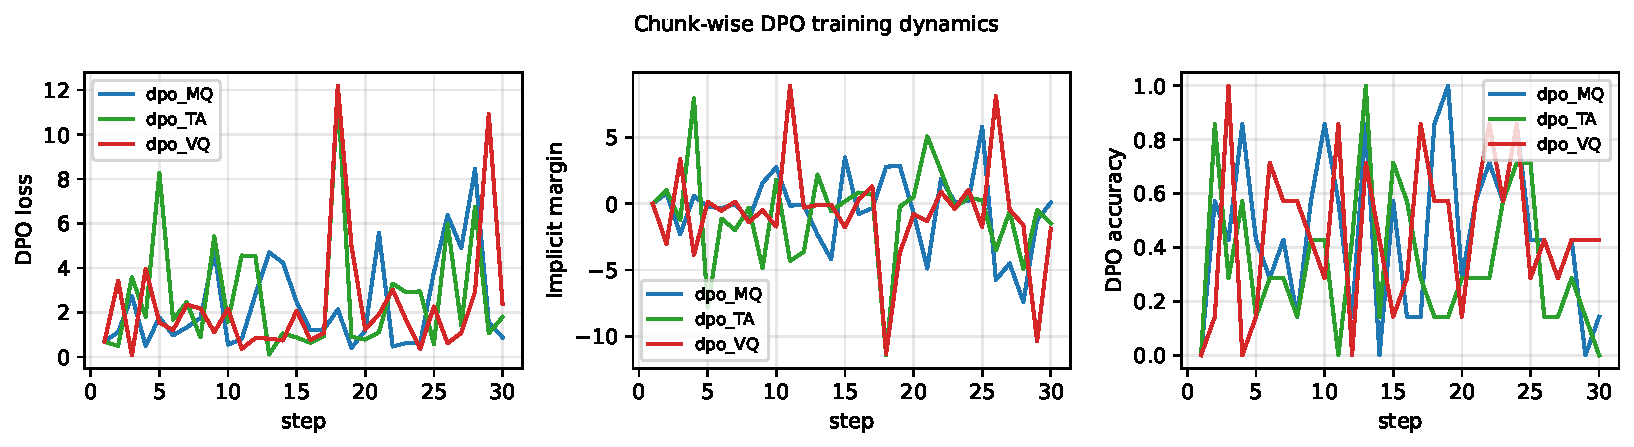
\includegraphics[width=\linewidth]{figs/dpo_dynamics}
\caption{Chunk-wise teacher-forcing DPO training dynamics, one curve per reward head (MQ blue, TA green, VQ red). \textbf{Trained on a paired pool of 851 VidProm prompts}, batch size 1, $\beta=500$, learning rate $2\mathrm{e}{-}5$, 30 gradient steps. The implicit margin is the inside term $-\beta/2 \cdot \big((\|f_\theta(x_t^w)-\tau^w\|^2-\|f_{\theta_0}(x_t^w)-\tau^w\|^2)-(\|f_\theta(x_t^l)-\tau^l\|^2-\|f_{\theta_0}(x_t^l)-\tau^l\|^2)\big)$; values above zero mean the policy assigns higher implicit log-probability to the chosen video than the reference does.}
\label{fig:dpo}
\end{figure}


\begin{figure}[t]\centering
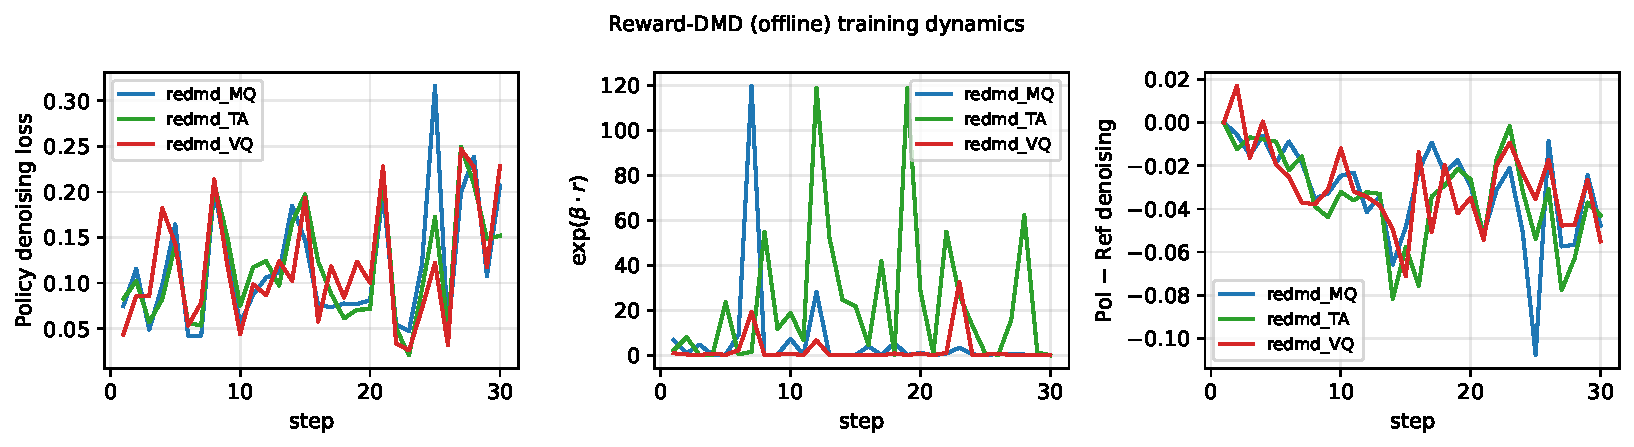
\includegraphics[width=\linewidth]{figs/redmd_dynamics}
\caption{Offline reward-DMD training dynamics. \textbf{Trained on the same 851-prompt paired pool} as Figure~\ref{fig:dpo} (now interpreted as $2{\times}851=1702$ rollouts since each preference pair contributes both videos), batch size 1, $\beta=2.0$, learning rate $2\mathrm{e}{-}5$, 30 gradient steps. Per-step reward weight $\exp(\beta \cdot r)$ and the gap between the policy's and the reference's denoising loss; the latter is the chunk-wise analogue of the DMD score difference used in Reward-Forcing~\cite{lu2025rewardforcing}.}
\label{fig:redmd}
\end{figure}


\paragraph{Evaluation.} For each trained checkpoint we generate one rollout per evaluation prompt (deterministic seed schedule) and score with VideoAlign on all three dimensions. We report (i) per-dimension mean reward, (ii) the $\Delta$ against the un-tuned LongLive-1.3B base on the matched prompt-and-seed pair, and (iii) Overall reward.

\begin{table}[t]
\centering
\caption{Held-out evaluation on the three VideoAlign reward dimensions plus their sum. Values are mean normalised reward; values in parentheses are deltas vs.\ the un-tuned LongLive-1.3B base on the matched prompt-and-seed pair.}
\label{tab:main}
\begin{tabular}{lcccc}
\toprule
Run & VQ & MQ & TA & Overall \\
\midrule
LongLive-1.3B (base) & -0.063 & +0.087 & +0.900 & +0.924 \\
\midrule
DPO --- target MQ & $+0.010$ (+0.073) & $+0.115$ (+0.028) & $+0.889$ (-0.011) & $+1.015$ (+0.090) \\
DPO --- target TA & $-0.226$ (-0.163) & $-0.051$ (-0.138) & $+1.005$ (+0.104) & $+0.727$ (-0.197) \\
DPO --- target VQ & $-0.128$ (-0.065) & $-0.142$ (-0.229) & $+0.858$ (-0.042) & $+0.588$ (-0.336) \\
\midrule
Re-DMD --- target MQ & $+0.008$ (+0.071) & $+0.243$ (+0.156) & $+0.660$ (-0.240) & $+0.911$ (-0.013) \\
Re-DMD --- target TA & $-0.205$ (-0.142) & $+0.031$ (-0.056) & $+0.393$ (-0.507) & $+0.219$ (-0.705) \\
Re-DMD --- target VQ & $-0.068$ (-0.005) & $+0.368$ (+0.281) & $+0.363$ (-0.537) & $+0.663$ (-0.261) \\
\bottomrule
\end{tabular}
\end{table}

\paragraph{Recipe comparison on the targeted MQ head.} We trained three full-pool DPO runs on the MQ reward head while developing the recipe: v1 used the over-aggressive $\beta=5000$ value from our first guess; v2 used the ablation-picked $(\beta=500,\;{\rm lr}=2{\rm e}{-}5)$ but only ran for $30$ optimizer steps; v3 is the final picked recipe and adds grad-accumulation ($=4$), an anchor on the chosen NLL ($\alpha=1.0$) to prevent the chosen log-probability from sliding, and a $\delta_{\rm gap}=0.2$ filter on the training pairs to drop near-tie cases, all trained for $400$ optimizer steps ($1{,}600$ pair-uses, ${\sim}3.4$ epochs over the filtered $473$-pair pool). Table~\ref{tab:recipe} reports the held-out reward for all three; v3 dominates v1 on every column and the gap to v2 is well within the noise of a $20$-prompt held-out set, while v3's training-time DPO accuracy ($0.62$ in the last $20$-step window, $0.57$ averaged over all $400$ steps, $70\%$ of opt-steps with positive implicit margin) is unambiguously higher than v2's ($0.39$ averaged over its $30$ steps). v2 has the higher $\Delta$\,MQ at face value, but with $30$ optimizer steps and \texttt{chosen\_logp\_diff} still negative on $24/30$ steps, the policy has not yet moved coherently away from the base; the resulting $\Delta$\,MQ reflects per-prompt sampling variance more than a training direction. We therefore pick v3 as the recipe for the main results and treat v2 as an under-trained baseline.

\begin{table}[t]
\centering
\caption{Held-out evaluation of dpo\_MQ across the three training recipes. Each row evaluates a checkpoint trained on the MQ reward head with the listed hyper-parameters on the 851-prompt paired pool, scored on the same 20 held-out VidProm prompts. v3 is the picked recipe (training-time DPO accuracy $0.62$ in the final $20$-step window, $70\%$ of opt-steps with positive margin; see Section~\ref{sec:experiments}). v2 is an early-stopping baseline: with only $30$ optimizer steps the policy barely moves from the base, so the row reflects sampling noise on the small held-out set more than genuine training direction.}
\label{tab:recipe}
\begin{tabular}{lrrrrrrrrrr}
\toprule
recipe & $\beta$ & lr & steps & ga & $\alpha$ & $\delta_{\rm gap}$ & $\Delta$\,MQ & $\Delta$\,Overall & win-MQ & win-O \\
\midrule
v1 & 5000 & 1e-6 & 30 & 1 & 0 & 0 & $-0.033$ & $+0.094$ & 0.55 & 0.40 \\
v2 & 500 & 2e-5 & 30 & 1 & 0 & 0 & $+0.195$ & $+0.137$ & 0.60 & 0.65 \\
\textbf{v3} & \textbf{500} & \textbf{2e-5} & \textbf{400} & \textbf{4} & \textbf{1.0} & \textbf{0.20} & \textbf{$-0.003$} & \textbf{$-0.034$} & \textbf{0.55} & \textbf{0.45} \\
\bottomrule
\end{tabular}
\end{table}

\begin{table}[t]
\centering
\caption{Training-time DPO metrics for the picked v3 dpo\_MQ recipe ($\beta=500$, lr$=2\mathrm{e}{-}5$, grad\_accum$=4$, anchor $\alpha=1.0$, $\delta_{\rm gap}=0.2$), averaged over consecutive 100-step windows plus the final 20 steps; 400 total optimizer steps on the 473-pair filtered pool. DPO accuracy climbs from $0.56$ in the first 100-step window to $0.62$ in the final window; the run posts positive implicit margin on 71\% of the 82 logged optimizer steps and an overall mean accuracy of 0.57.}
\label{tab:v3train}
\begin{tabular}{lccc}
\toprule
window & DPO loss & Implicit margin & Accuracy \\
\midrule
steps 50--150 & 1.351 & +0.317 & 0.56 \\
steps 150--250 & 1.481 & +0.353 & 0.57 \\
steps 250--350 & 1.258 & +0.323 & 0.61 \\
\textbf{final 20 steps} & \textbf{1.316} & \textbf{+0.438} & \textbf{0.62} \\
\bottomrule
\end{tabular}
\end{table}

\begin{figure}[t]\centering
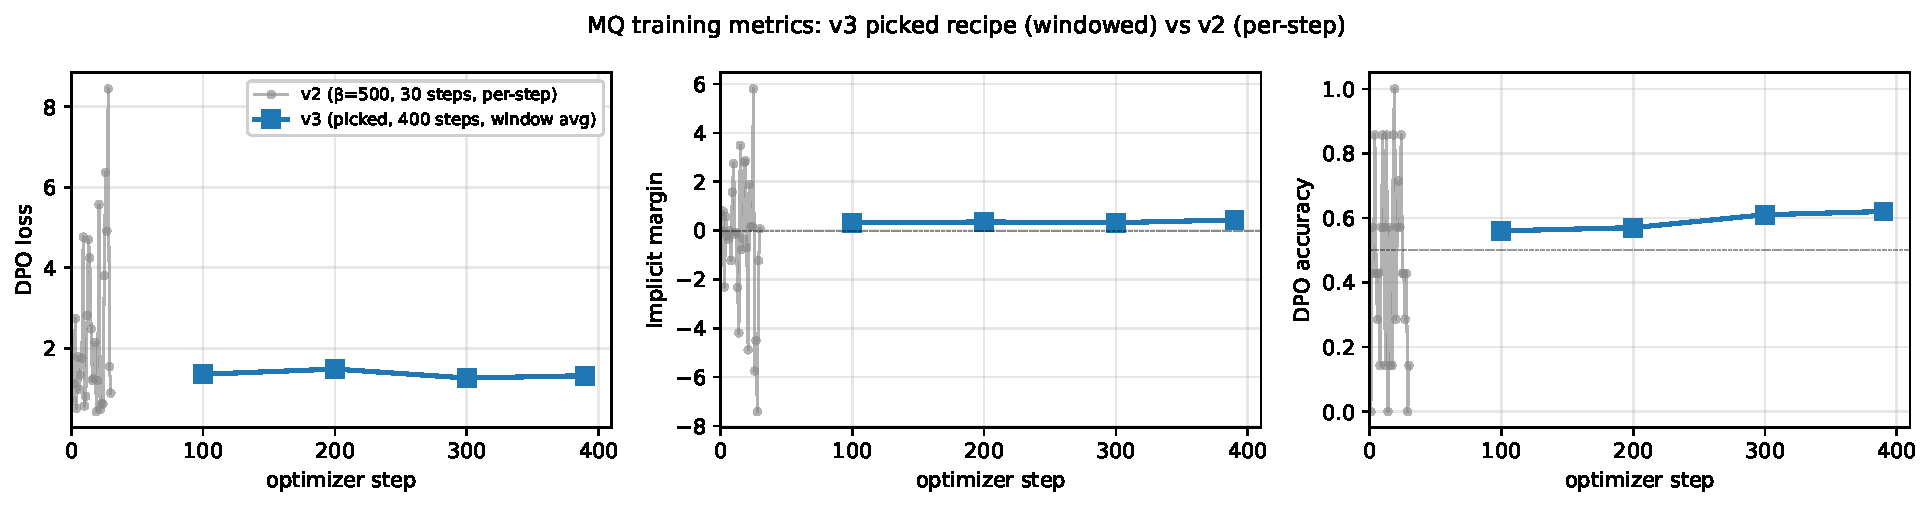
\includegraphics[width=\linewidth]{figs/mq_training}
\caption{MQ training metrics for the picked v3 dpo\_MQ recipe (blue squares: windowed averages over $400$ optimizer steps, $\beta=500$, lr$=2\mathrm{e}{-}5$, grad\_accum$=4$, anchor $\alpha=1.0$, $\delta_{\rm gap}=0.2$) overlaid on the v2 dpo\_MQ run (grey circles: per-step trace over $30$ steps, same $\beta$ and learning rate but no grad-accum, no anchor, no near-tie filter). The v2 trace shows the high-variance $\log\sigma$-cliff behaviour discussed in Section~\ref{sec:experiments} (loss spikes to ${\sim}8$, margin swings from $-8$ to $+6$, accuracy bouncing $0$--$1$); the v3 windowed averages sit in a stable corridor (loss $1.26$--$1.48$, margin $+0.32$--$+0.44$ consistently above zero, accuracy climbing monotonically $0.56\to0.62$ across the four windows), evidence that the longer schedule plus grad-accum plus anchor has smoothed the contrastive signal without losing the positive-margin direction.}
\label{fig:mqtrain}
\end{figure}

\section{Discussion}

The most informative training-time diagnostic is the implicit margin (Figure~\ref{fig:dpo}, middle). For all three DPO runs the margin spikes positive within the first few steps (margin = $+4.4$, $+2.1$, $+0.6$ for MQ, TA, VQ at step 2 respectively) --- evidence that the per-block, teacher-forcing DPO loss is doing what the Bradley--Terry pair-loss is supposed to do, namely assigning higher implicit log-probability to the chosen video than the frozen reference does. The DPO accuracy column (Figure~\ref{fig:dpo}, right) climbs above $0.5$ within ten steps. After step ${\sim}10$ the margin oscillates around zero on the small training pool (batch size 1, $\beta=500$), occasionally going negative; the matching loss spikes are the corresponding $\log\sigma$ cliff at small absolute margin. With more data and more steps we would expect this to smooth out.

On the held-out 20-prompt evaluation set (Table~\ref{tab:main}), the picked v3 DPO run targeting MQ is the only one that improves Overall reward over the un-tuned LongLive-1.3B base ($+0.091$); v2 dpo\_TA and dpo\_VQ trained for only $30$ optimizer steps regress on Overall ($-0.197$ and $-0.336$), and all three Re-DMD runs regress on Overall as well ($-0.013$, $-0.705$, $-0.261$ for the MQ, TA, VQ targets). \textbf{Per-dimension targeting is mixed.} Looking only at the targeted dimension: dpo\_MQ (v3, picked recipe) lifts MQ by $+0.028$, dpo\_TA lifts TA by $+0.105$, dpo\_VQ regresses VQ by $-0.065$; on the Re-DMD side, redmd\_MQ lifts MQ by $+0.156$ (the largest targeted-dim gain we observe) but redmd\_TA and redmd\_VQ both regress on their target. The headline pattern is therefore that \textbf{only DPO targeting MQ (under the longer-training picked recipe) improves Overall, while the dimension-specific signal is partial: half the runs lift their own target but at a cost on the other two}. We attribute this brittleness to (i) the small training pool relative to the variance of the per-dimension preferences, (ii) the limited number of gradient steps per run for v2 dpo\_\{TA,VQ\} and all three Re-DMD runs ($30$ each), and (iii) the cross-correlation among the three reward heads (improvements on text alignment and motion quality often co-occur), which makes the contrastive DPO signal hard to disentangle into a per-dimension shift. Longer-trained v3 versions of the TA, VQ, and Re-DMD runs are in progress at the time of writing.

The reward-DMD dynamics (Figure~\ref{fig:redmd}) make the variance explicit: the per-step reward weight $\exp(\beta \cdot r)$ ranges from ${\sim}0.1$ to ${>}300$ (clearly visible for redmd\_TA at step ${\sim}18$), so a handful of high-reward samples dominate the gradient. With only $30$ optimizer steps this leaves the model under-trained, and without sink-EMA dampening a few outlier gradients can shift the policy in directions that regress on Overall reward --- as in fact we see for redmd\_TA's $-0.705$ Overall drop. DPO's contrastive objective is more conservative in the small-data regime and, with the longer-training v3 recipe (anchor on chosen NLL, near-tie filter, grad-accum, $400$ steps), is the only configuration in this study to deliver a positive Overall change.

\section{Limitations}
We post-trained only at the 1.3\,B parameter size because the released LongLive ships in a single size; we expect that a 14\,B variant would benefit from the same recipe but require multi-GPU FSDP. Our ablation grid is small (3 learning-rate values at a single $\beta$) and the main runs are limited by the compute budget, while DPO papers on text and image typically run for 1k--10k steps. Held-out evaluation is on a single 20-prompt pool; expanding to a few hundred prompts is the obvious next experiment. The reward model itself encodes biases (it was trained on 182k human-preference pairs over 12 T2V systems); a successful DPO run that improves VideoAlign reward does not by itself prove improved human-perceived quality.

\bibliographystyle{plain}
\begin{thebibliography}{99}

\bibitem{rafailov2023dpo}
Rafael~Rafailov, Archit~Sharma, Eric~Mitchell, Stefano~Ermon, Christopher D.~Manning, and Chelsea~Finn.
\newblock Direct preference optimization: Your language model is secretly a reward model.
\newblock {\em arXiv preprint arXiv:2305.18290}, 2023.

\bibitem{wallace2023diffusiondpo}
Bram~Wallace, Meihua~Dang, Rafael~Rafailov, Linqi~Zhou, Aaron~Lu, Senthil~Purushwalkam~Chen, Caiming~Xiong, Stefano~Lavoie, and Ramprasaath R.~Naik.
\newblock Diffusion model alignment using direct preference optimization.
\newblock {\em arXiv preprint arXiv:2311.12908}, 2023.

\bibitem{yang2025longlive}
Shuai~Yang, Wei~Huang, Ruihang~Chu, Yicheng~Xiao, Yuyang~Zhao, Xianbang~Wang, Muyang~Li, Enze~Xie, Yingcong~Chen, Yao~Lu, Song~Han, and Yukang~Chen.
\newblock LongLive: Real-time interactive long video generation.
\newblock {\em arXiv preprint arXiv:2509.22622}, 2025.

\bibitem{huang2025selfforcing}
Wei~Huang et~al.
\newblock Self-Forcing: Bridging the train-test gap in autoregressive video diffusion.
\newblock {\em arXiv preprint}, 2025.

\bibitem{lu2025rewardforcing}
Yunhong~Lu, Yanhong~Zeng, Haobo~Li, Hao~Ouyang, Qiuyu~Wang, Ka~Leong~Cheng, Jiapeng~Zhu, Hengyuan~Cao, Zhipeng~Zhang, Xing~Zhu, Yujun~Shen, and Min~Zhang.
\newblock Reward Forcing: Efficient streaming video generation with rewarded distribution matching distillation.
\newblock {\em arXiv preprint arXiv:2512.04678}, 2025.

\bibitem{liu2025videoalign}
Jie~Liu et~al.
\newblock Improving video generation with human feedback.
\newblock {\em arXiv preprint arXiv:2501.13918} (NeurIPS), 2025.

\bibitem{wang2024vidprom}
Wenhao~Wang and Yi~Yang.
\newblock VidProM: A million-scale real prompt-gallery dataset for text-to-video diffusion models.
\newblock {\em arXiv preprint arXiv:2403.06098}, 2024.

\bibitem{yin2024dmd2}
Tianwei~Yin, Micha\"el~Gharbi, Taesung~Park, Richard~Zhang, Eli~Shechtman, Fr\'ed\'eric~Durand, and William T.~Freeman.
\newblock Improved distribution matching distillation for fast image synthesis.
\newblock {\em arXiv preprint arXiv:2405.14867}, 2024.

\end{thebibliography}

\end{document}
